\documentclass{beamer}

\mode<presentation> {
\usetheme{Malmoe} 
\usecolortheme{beaver} 
}

\usepackage{graphicx} 
\usepackage{booktabs} 
\usepackage{amsmath}
\usepackage{graphicx}
\usepackage[colorinlistoftodos]{todonotes}
\usepackage{hyperref}
\usepackage{multimedia}
\usepackage{multirow,tabularx}
\usepackage{media9}
\usepackage{tikz}
\usetikzlibrary{calc,positioning}
\usepackage{xcolor}
\hypersetup{
    colorlinks=true,       
    linkcolor=blue,          
    citecolor=blue,        
    urlcolor=blue           
}
%----------------------------------------------------------------------------------------
%	TITLE PAGE
%----------------------------------------------------------------------------------------

\title[CPS]{\textcolor{black}{{Resilient Asymptotic Consensus in Robust Networks \cite{p1}}}} 
\subtitle[]{}

\author{Jedediah Fry, George Kontoudis}
\institute[VT] 
{Midterm\\
AOE5984 Cyber-Physical Systems and Distributed Control\\
Spring 2017\\
\medskip
\it{Aerospace and Ocean Engineering Department, Virginia Tech} 
}
\date{\today}

\setbeamertemplate{footline}[text line]{%
  \parbox{\linewidth}{\vspace*{-8pt}\today 
  \hfill\insertshortsubtitle
  \hfill\insertpagenumber}}
\setbeamertemplate{navigation symbols}{}

\begin{document}

\begin{frame}[plain]
\titlepage 
\end{frame}

\begin{frame}
\frametitle{Outline} 
\tableofcontents 
\end{frame}

%----------------------------------------------------------------------------------------
%	PRESENTATION SLIDES
%----------------------------------------------------------------------------------------
%------------------------------------------------
\section{Introduction}
%------------------------------------------------

\begin{frame}
\frametitle{Introduction}

\end{frame}

%------------------------------------------------
\section{Problem Formulation}
%------------------------------------------------

\begin{frame}
\frametitle{Problem Formulation}

\end{frame}

%------------------------------------------------
\section{Consensus Algorithm}
%------------------------------------------------

\begin{frame}
\frametitle{Consensus Algorithm}

\end{frame}

%------------------------------------------------
\section{Robust Network Topologies}
%------------------------------------------------

\begin{frame}
\frametitle{Robust Network Topologies}

\end{frame}

%------------------------------------------------
\section{Resilient Consensus Analysis}
%------------------------------------------------

\begin{frame}
\frametitle{Resilient Consensus Analysis}
\begin{itemize}
\item W-MSR always satisfies safety condition for RAC 
\item $M[t]$, $m[t]$ maximum \& minimum values of normal nodes $i \in N$ \vspace{.2cm}
\end{itemize}

\textbf{\textit{Lemma}}: Regardless of network topology, for each normal node $i \in N$ we get
\begin{equation*}
x_i[t+1] \in [m(t),M(t)],
\end{equation*}
when using W-MSR algorithm w/ parameter F or $f$ under F-local, F-total or $f$-fraction (Byzantine or malicious) models.
\end{frame}
%------------------------------------------------

\begin{frame}
\frametitle{F-Total Malicious Model}
\begin{itemize}
\item Characterize networks by necessary \& sufficient conditions of W-MSR to succeed
\end{itemize}
\begin{table}
\centering
\begin{tabular}{|c|c|c|c|c|}
\hline \scriptsize{\textbf{Time-}} &\scriptsize{\textbf{Threat Models}} &  \scriptsize{\textbf{Scope}} & \scriptsize{\textbf{Necessary}} & \scriptsize{\textbf{Sufficient}} \\
\hline \scriptsize{Invariant} &\scriptsize{Malicious} & \scriptsize{F-Total}  & \scriptsize{(F+1,F+1)-robust} & \scriptsize{(F+1,F+1)-robust} \\
\hline \scriptsize{Variant} &\scriptsize{Malicious} & \scriptsize{F-Total}  & \scriptsize{-} & \scriptsize{(2F+1)-robust}  \\
\hline
\end{tabular}
\end{table}
\end{frame}
%------------------------------------------------

\begin{frame}
\frametitle{F-Local Malicious Model}
\begin{itemize}
\item Employ F-Local when total number of adversaries is large in large-scale networks
\end{itemize}
\begin{table}
\centering
\begin{tabular}{|c|c|c|c|c|}
\hline \scriptsize{\textbf{Time-}} &\scriptsize{\textbf{Threat Models}} &  \scriptsize{\textbf{Scope}} & \scriptsize{\textbf{Necessary}} & \scriptsize{\textbf{Sufficient}} \\
\hline \scriptsize{Invariant} &\scriptsize{Malicious} & \scriptsize{F-Local}  & \scriptsize{(F+1)-robust} & \scriptsize{(2F+1)-robust} \\
\hline \scriptsize{Variant} &\scriptsize{Malicious} & \scriptsize{F-Local}  & \scriptsize{-} & \scriptsize{(2F+1)-robust}  \\
\hline
\end{tabular}
\end{table}
\begin{itemize}
\item For every $F \in \mathbb{Z}_{>0}$ there exists a 2F-robust network that fails to reach consensus w/ W-MSR
\end{itemize}
\end{frame}
%------------------------------------------------

\begin{frame}
\frametitle{$f$-Fraction Local Malicious Model}
\begin{itemize}
\item Characterize networks by necessary \& sufficient conditions of W-MSR to succeed
\end{itemize}
\begin{table}
\centering
\begin{tabular}{|c|c|c|c|c|}
\hline \scriptsize{\textbf{Time-}} &\scriptsize{\textbf{Threat Models}} &  \scriptsize{\textbf{Scope}} & \scriptsize{\textbf{Necessary}} & \scriptsize{\textbf{Sufficient}} \\
\hline \multirow{2}{*}{\scriptsize{Invariant}} & \multirow{2}{*}{\scriptsize{Malicious}} & \scriptsize{$f$-Fraction}  & \scriptsize{$p^{\prime}$-fraction robust,} & \scriptsize{$p$-fraction robust, } \\
& & \scriptsize{Local}  & \scriptsize{$2f\leq p\leq 1$} & \scriptsize{ $2f\leq p\leq 1$}\\ 
\hline \multirow{2}{*}{\scriptsize{Variant}} & \multirow{2}{*}{\scriptsize{Malicious}} & \scriptsize{$f$-Fraction}  & \multirow{2}{*}{\scriptsize{-}} & \scriptsize{$p$-fraction robust, } \\
& & \scriptsize{Local}  &  & \scriptsize{$2f< p\leq 1$}\\
\hline
\end{tabular}
\end{table}

\end{frame}
%------------------------------------------------

\begin{frame}
\frametitle{Byzantine Threat Models}
\begin{table}
\centering
\begin{tabular}{|c|c|c|c|c|}
\hline \scriptsize{\textbf{Time-}} &\scriptsize{\textbf{Threat Models}} &  \scriptsize{\textbf{Scope}} & \scriptsize{\textbf{Necessary}} & \scriptsize{\textbf{Sufficient}} \\
\hline \multirow{2}{*}{\scriptsize{Invariant}} & \multirow{2}{*}{\scriptsize{Byzantine}} & \scriptsize{F-Total \&}  & \scriptsize{Normal Network} & \scriptsize{Normal Network} \\
& & \scriptsize{F-Local}  & \scriptsize{(F+1)-robust} & \scriptsize{(F+1)-robust}\\ 
\hline \multirow{2}{*}{\scriptsize{Invariant}} & \multirow{2}{*}{\scriptsize{Byzantine}} & \scriptsize{$f$-Fraction}  & \scriptsize{Normal Network} & \scriptsize{Normal Network} \\
& & \scriptsize{Local}  & \scriptsize{$f$-robust} & \scriptsize{$p$-robust, $p>f$}\\
\hline \multirow{2}{*}{\scriptsize{Variant}} & \multirow{2}{*}{\scriptsize{Byzantine}} & \scriptsize{F-Total \&}  & \multirow{2}{*}{-} & \scriptsize{Normal Network} \\
& & \scriptsize{F-Local}  &  & \scriptsize{(F+1)-robust}\\ 
\hline \multirow{2}{*}{\scriptsize{Variant}} & \multirow{2}{*}{\scriptsize{Byzantine}} & \scriptsize{$f$-Fraction}  & \multirow{2}{*}{-} & \scriptsize{Normal Network} \\
& & \scriptsize{Local}  &  & \scriptsize{$p$-robust, $2f< p\leq 1$}\\
\hline
\end{tabular}
\end{table}
\begin{itemize}
\item Normal network $D_N$, induced by normal nodes
\end{itemize}
\end{frame}

%------------------------------------------------
\section{Simulations}
%------------------------------------------------

\begin{frame}
\frametitle{Simulation Network Topology}
\begin{itemize}
\item For a given (2,2)-robust network we can sustain 1-Total malicious threat model 
\end{itemize}
\begin{figure}[!h]
	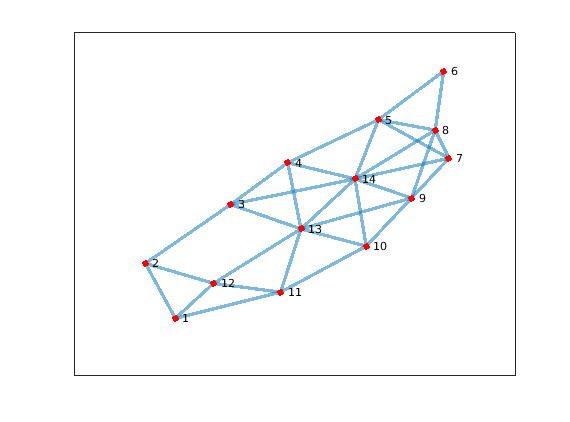
\includegraphics[scale=0.50]{figures/simulationGraph.png}
	\centering
\end{figure}
\end{frame}

%------------------------------------------------

\begin{frame}
\frametitle{LCP algorithm}
\begin{columns}[c] % The "c" option specifies centered vertical alignment while the "t" option is used for top vertical alignment

\column{.57\textwidth} 
The Linear Consensus Protocol (LCP) is given by
\begin{equation*}
x_i(t+1)=\sum_{j\in J_i(t)}w_{ij}(t)x^{j}_{i}(t)
\end{equation*}
\begin{itemize}
\item $\sum_{j=1}^n w_{ij}(t)=1$
\item $J_i(t)=V_i(t)\cup \{i\}$
\item $x_1(t+1)= w_{1,1}x_1+w_{1,2}x_2+w_{1,11}x_{11}+w_{1,12}x_{12}$
\end{itemize}

    
\column{.49\textwidth} 
    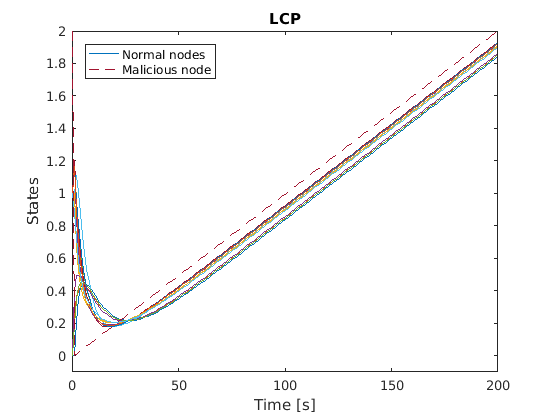
\includegraphics[scale=0.40]{figures/LCP.png}
	\centering
\end{columns}

\end{frame}

%------------------------------------------------

\begin{frame}
\frametitle{W-MSR algorithm}
\begin{columns}[c] % The "c" option specifies centered vertical alignment while the "t" option is used for top vertical alignment

\column{.57\textwidth} 
The W-MSR algorithm is given by
\begin{equation*}
x_i(t+1)=\sum_{j\in J_i(t)\backslash R_i(t)}w_{ij}(t)x^{j}_{i}(t)
\end{equation*}
\begin{itemize}
\item $R_i(t)$ denotes the reduced nodes
\item Using F=1 because we have 1-Total model
\end{itemize}

    
\column{.49\textwidth} 
    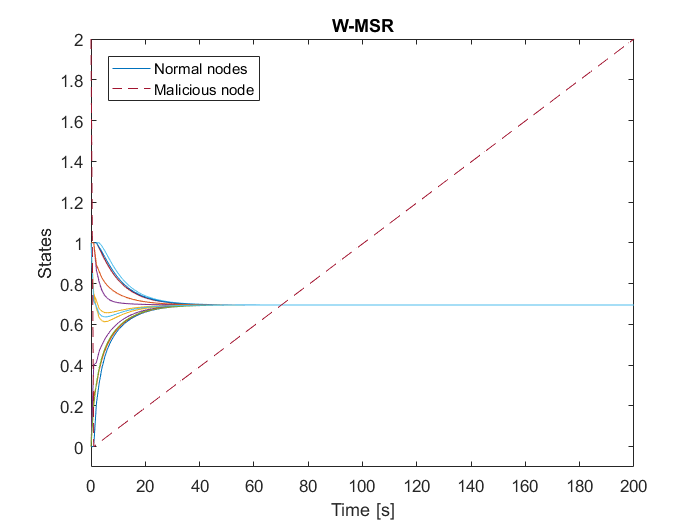
\includegraphics[scale=0.32]{figures/W_MSR.png}
	\centering
\end{columns}

\end{frame}

%------------------------------------------------

\begin{frame}
\frametitle{Node removal W-MSR}
The following update law applies w/ W-MSR algorithm
\begin{table}
\centering
\begin{tabular}{|c|c|c|c|c|}
\hline \scriptsize{\textbf{Node}} &\scriptsize{\textbf{Sort List}} & \scriptsize{\textbf{Step}}&  \scriptsize{\textbf{Values}}  & \scriptsize{\textbf{Removed}} \\
\hline \scriptsize{1} &\scriptsize{\{1, 2, 11, 12\} } & \scriptsize{0}& \scriptsize{\{0, 0, 0, 0\}}   & \scriptsize{-} \\
\hline \scriptsize{1} &\scriptsize{\{1, 2, 11, 12\} } & \scriptsize{1}& \scriptsize{\{0, 0.25, 0.4, 0.2\}}   & \scriptsize{\{11\} } \\
\hline \scriptsize{1} &\scriptsize{\{1, 2, 11, 12\}} & \scriptsize{6}& \scriptsize{\{0.4453, 0.4322, 0.4649, 0.4553\}}   & \scriptsize{\{2, 11\}} \\	
\hline \scriptsize{10} &\scriptsize{\{9, 10, 11, 13, 14\} } & \scriptsize{0}& \scriptsize{\{1, 1, 0, 1, 2\}}   & \scriptsize{\{11, 14\}} \\
\hline \scriptsize{10} &\scriptsize{\{9, 10, 11, 13, 14\} } & \scriptsize{1}& \scriptsize{\{1.167, 1, 0.4, 0.87, 0\}}   & \scriptsize{\{9, 14\}} \\
\hline \scriptsize{10} &\scriptsize{\{9, 10, 11, 13, 14\} } & \scriptsize{30} & \scriptsize{\{0.7, 0.6921, 0.68, 0.6935, 0.28\}}  & \scriptsize{\{13, 14\}} \\	
\hline
\end{tabular}
\end{table}

\end{frame}

%------------------------------------------------
\section{Construction \& Properties of Robust Digraphs}
%------------------------------------------------

\begin{frame}
\frametitle{Construction of Robust Digraphs}
\textbf{\textit{Theorem}}: Let $D=(V, \mathcal{E} )$ be an $(r,s)$-robust digraph, $S\in \mathbb{Z}_{>0}$. Then, $D^{\prime}=(V\cup \{v_{new}\},\mathcal{E} \cup \{\varepsilon_{new} \})$ is $(r,s)$-robust if
\begin{equation*}
d_{v_{new}}^{in}\geq r+s-1,
\end{equation*}
where $v_{new}$ is the new vertex added to $D$, and $\varepsilon_{new}$ is the directed edge set related to $v_{new}$, 
\begin{itemize}
\item Start w/ an $(r,s)$-robust digraph 
\item Add new nodes w/ incoming edges at least $r+s-1$
\item Arbitrary node selection, scale-free networks
\end{itemize}

\end{frame}

%------------------------------------------------

\begin{frame}
\frametitle{Robust Digraph Example}

\begin{columns}[c] % The "c" option specifies centered vertical alignment while the "t" option is used for top vertical alignment

\column{.65\textwidth} 
\begin{itemize}
\item Start w/ a $K_5$ graph (complete-fully connected on 5 nodes)
\item $K_5$ is the only $(3,2)$-robust 5 node digraph 
\item Add new nodes w/ incoming edges w/ at least $r+s-1=3+2-1=4$
\item End up w/ a $(3,2)$-robust 10 node digraph, also $4$-robust
\end{itemize}

    
\column{.45\textwidth} 
    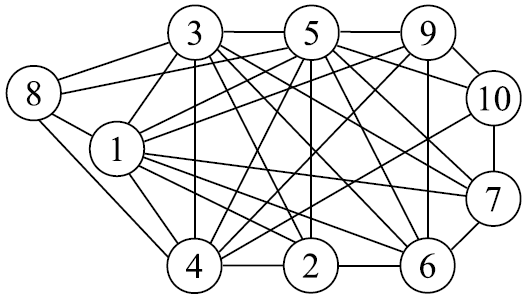
\includegraphics[scale=0.38]{figures/RobustDigraph.png}
	\centering \\
	\cite{p1}
\end{columns}


\end{frame}

%------------------------------------------------


\begin{frame}
\frametitle{Robust Digraph Illustration}
\begin{columns}[t]
\column{.30\textwidth} 
    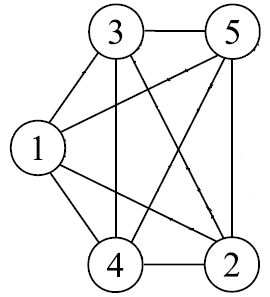
\includegraphics[scale=0.32]{figures/RobustDigraph0.png}
	\centering \\	
\column{.35\textwidth} 
    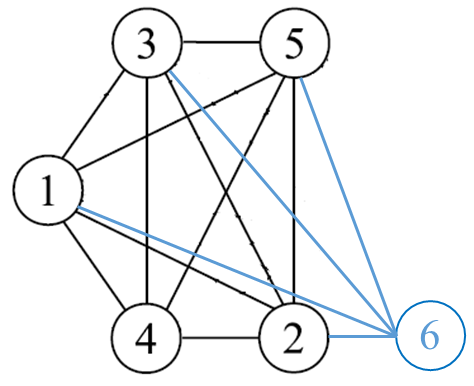
\includegraphics[scale=0.25]{figures/RobustDigraph1.png}
	\centering \\
\column{.35\textwidth} 
    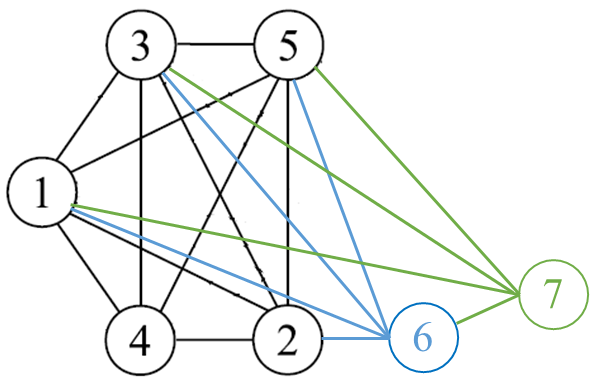
\includegraphics[scale=0.25]{figures/RobustDigraph2.png}
	\centering \\
\end{columns}
\vspace{.5cm}
\begin{columns}[t]	
\column{.35\textwidth} 
    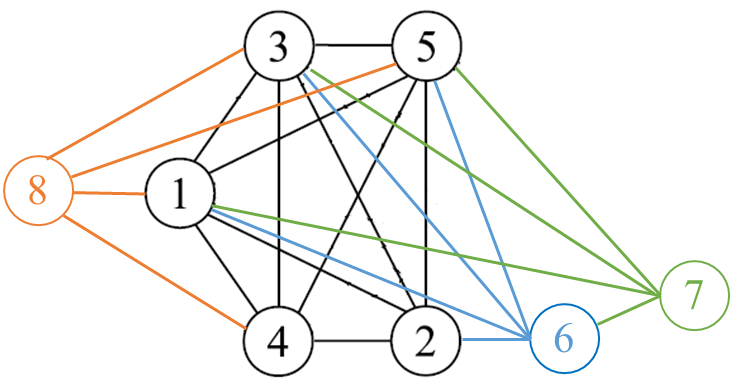
\includegraphics[scale=0.25]{figures/RobustDigraph3.png}
	\centering \\  
\column{.35\textwidth} 
    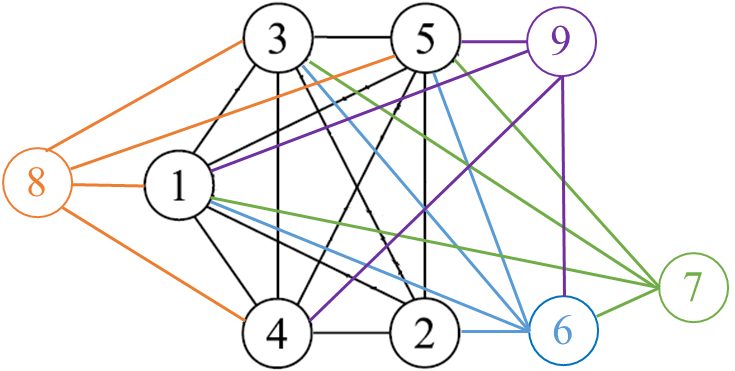
\includegraphics[scale=0.25]{figures/RobustDigraph4.png}
	\centering \\	
\column{.35\textwidth} 
    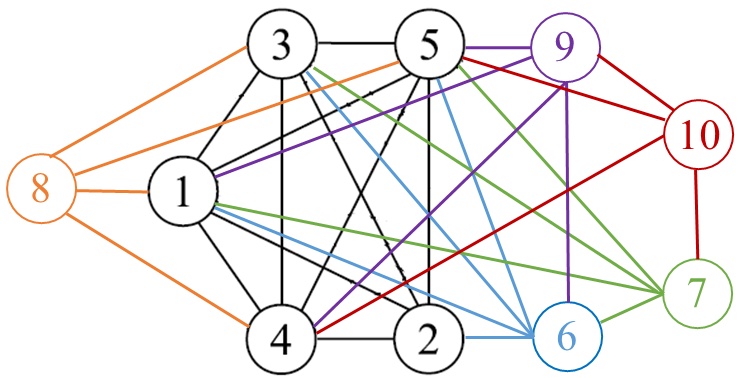
\includegraphics[scale=0.25]{figures/RobustDigraph5.png}
	\centering \\
\end{columns}

\end{frame}

%------------------------------------------------

\begin{frame}
\frametitle{Properties of Robust Networks (1/2)}
\textbf{\textit{Observation}}: $(r,1)$-robustness $\equiv$ $r$-robustness\\
\vspace{.2cm}
\textbf{\textit{Lemma}}: Every $(r,s)$-robust digraph $D=(V, \mathcal{E} )$ is also $(r^{\prime},s^{\prime})$-robust when $0\leq r^{\prime}\leq r$, $1\leq s^{\prime}\leq s$.\\
\vspace{.2cm}
\textbf{\textit{Lemma}}: Suppose digraph $D=(V, \mathcal{E} )$ is  $(r,s)$-robust, spanning  $D^{\prime}=(V, \mathcal{E}^{\prime})$, where $\mathcal{E}^{\prime}=\mathcal{E}\cup \mathcal{E}^{\prime \prime}$ and $|\mathcal{E}^{\prime \prime}|\leq 0$. Then $D^{\prime}$ is $(r,s)$-robust.\\
\vspace{.2cm}
\textbf{\textit{Lemma}}: No digraph $D=(V, \mathcal{E} )$ on $n$ nodes is $([n/2]+1)$-robust. On the other hand, the complete digraph $K_n=(V, \mathcal{E}_{K_n} )$ is the only  $([n/2],s)$-robust for $1\leq s\leq n$ and n odd.

\end{frame}

%------------------------------------------------

\begin{frame}
\frametitle{Properties of Robust Networks (2/2)}
\textbf{\textit{Lemma}}: Given an $(r,s)$-robust digraph $D=(V, \mathcal{E} )$ w/ $0\leq r\leq [n/2]$ the minimum in-degree of $D$ is at least
\begin{equation*}
\delta^{in}(D)\geq \bigg\{
  \begin{matrix}
  r+s-1 & if \hspace{.2cm} s<r ;\\
  2r-2 & if \hspace{.2cm} s\geq r .
  \end{matrix}
\end{equation*}
\textbf{\textit{Lemma}}:  Given an $(r,s)$-robust ($p$-fraction robust) digraph $D$, let $D^{\prime}$ be the digraph produced by removing up to $k$ incoming edges from each node in $D$, where $0\leq k\leq r$ ($0\leq q< p\leq 1$). Then $D^{\prime}$ is $(r-k,s)$-robust ($(p-q)$-fraction robust).\\
\textbf{\textit{Theorem}}: Suppose $D=(V, \mathcal{E} )$ is an $r$-robust (or $(r,r)$-robust) digraph, w/ $0\leq r\leq [n/2]$ (or $3\leq r\leq [n/2]$). Then the underlying graph $G_D$ is at least $r$-connected (or $[3r/2]-1$-connected).
\end{frame}

%------------------------------------------------
\section{References}
%------------------------------------------------
\begin{frame}
\frametitle{References}
\footnotesize{
\begin{thebibliography}{99} % Beamer does not support BibTeX so references must be inserted manually as below

\bibitem[LeBlanc, 2013]{p1} H. LeBlanc, H. Zhang, X. Koutsoukos, S. Sundaram (2013)
\newblock Resilient asymptotic consensus in robust networks
\newblock \emph{IEEE Journal on Selected Areas in Communications, 31(4), 766-781}, 2013.

\end{thebibliography}
}
\end{frame}

%------------------------------------------------
\section{}
\begin{frame}
\begin{center}
\Huge {Thank You!}
\end{center}
\end{frame}

%----------------------------------------------------------------------------------------

\end{document} 